% @file           main.tex
% @brief          Template code of LaTeX
% @author         retact
% @date           2021-06-04 17:19:52
% $Version:       1.0
% @par            History
% - This src is released under the MIT License, see LICENSE.

\documentclass{jarticle}
\usepackage[dvipdfmx]{graphicx}%図表挿入のため
\usepackage[dvipdfmx]{color}%図表挿入のため
\usepackage{float}
\usepackage[top=30truemm,bottom=30truemm,left=25truemm,right=25truemm]{geometry}
 
% 全体のページ設定
% ページ番号をフッタにふる
\pagestyle{plain}

\makeatletter
 
\def\@thesis{〇〇実験}
\def\id#1{\def\@id{#1}}
\def\master#1{\def\@master{#1}}
\def\department#1{\def\@department{#1}}
 
\def\@maketitle{
\begin{center}
{\huge \@thesis \par} %修士論文と記載される部分
\vspace{10mm}
{\huge\bf \@title \par}% 論文のタイトル部分
\vspace{10mm}
{\Large 提出日 \@date\par} % 提出年月日部分
\vspace{20mm}
{\Large \@department \par} % 所属部分
\vspace{10mm}
{\Large \@master \par} % 学年部分
\vspace{10mm}
{\Large 学生番号 \@id \par} % 学籍番号部分
\vspace{10mm}
{\Large 氏名 \@author}% 氏名
\end{center}
%\par\vskip 1.5em
}
 
\makeatother
 
\title{Sample Title}
\date{\today}
\department{○○大学\\〇〇専攻}
\id{XXXXXXX}
\master{学士〇〇年}
\author{Sample Name}


% ------- ここから本文内容 ------------
\begin{document}
 
%%%%%%%%%%%%% 表紙 %%%%%%%%%%%%%%
\maketitle
\thispagestyle{empty} % ページ番号をなくす
\newpage% 改ページ

%%%%%%%%%%%%% 目次 %%%%%%%%%%%%%%
\setcounter{tocdepth}{2}
\tableofcontents
\newpage

%%%%%%%%%%%%% 3p %%%%%%%%%%%%%
\section{目的}
これは実験レポート用のサンプルテキストです。基本的な使い方を参考にしながらレポートを書いていきましょう。

\section{理論}
\subsection{表の出し方}
以下のような記述をすると以下のような表が出てきます。

% ----- 表:サンプル ------
\begin{table}[h]
 \caption{sample table}
 \label{table:SpeedOfLight}
 \centering
  \begin{tabular}{clll}
   \hline
   test1 & hogehoge & value  \\
   \hline \hline
   A & hogehoge & 0.25[m^3/min] \\
   B & hogehoge & 5.5[m]  \\
   C & hogehoge & 1800rpm(60Hz)  \\
      & hogehoge & 常温:0°C~40°C  \\
   \hline
  \end{tabular}
\end{table}
% --------------------

\subsection{画像の表示のさせ方}
以下のようにすると画像を表示させることができます。

% ----- 図:サンプル -----
\begin{figure}[h]%htbpのいずれかで指定
    \centering
   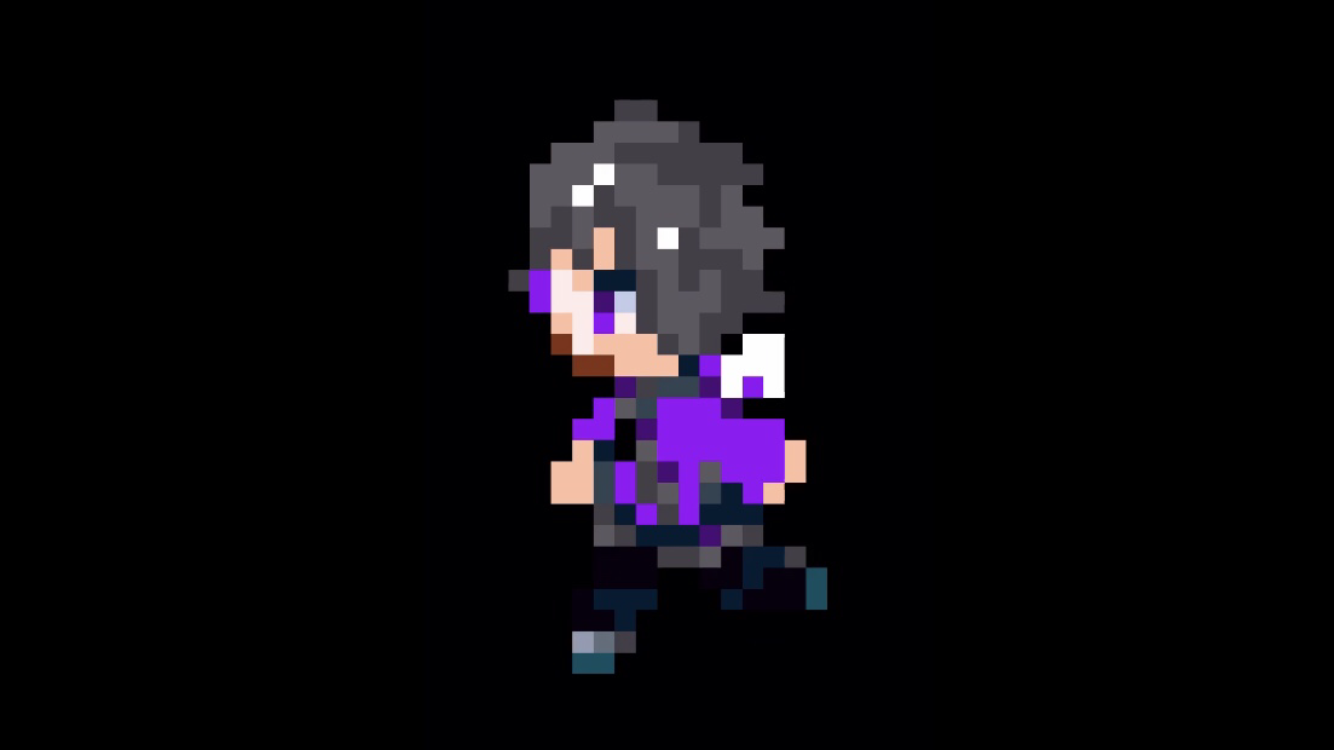
\includegraphics[width=80mm]{img/sample.png}
   \caption{sample image}
   \label{fig1}
\end{figure}
% -----------------------

\newpage% 改ページ

%%%%%%%%%%%% 4p %%%%%%%%%%%%%

\section{手法}
\subsection{実験装置}
\subsection{実験方法}
以下はsubsubsectionであり、subsectionの中をさらに小分けにすることができます。
\subsubsection{数式の挿入}
以下のようにすることで数式表示させることができます。
$$
\rho\left\{\frac{\partial v}{\partial t}+\nabla \cdot(\boldsymbol{v} \boldsymbol{v})\right\}=-\nabla p+\nabla \cdot(2 \mu \boldsymbol{D})
$$

\subsubsection{箇条書き}
以下のようにすることによって箇条書きをすることができます。
% ----- 箇条書き -----
\begin{quote}
 \begin{itemize}
  \item test1
  \item test2
  \item test
 \end{itemize}
\end{quote}
% ---------------------
\section{結果}
\subsection{ギリシャ文字}
以下のようにギリシャ文字を出力させる
$$A\rho\iota\sigma\tau{}o\tau\varepsilon\lambda\eta\varsigma$$




\section{考察}

\section{課題}
\subsection{〇〇〇〇}

\section{参考文献}
 
\end{document}